% \setlength{\parindent}{4em}
% \setlength{\parskip}{1em}
%%% Local Variables:
%%% mode: latex
%%% TeX-master: "IS1apuntes"
%%% End:

\section{Orientación a objetos}
\label{sec:org3620eb4}
\subsection{Enfoque estructurado}
\label{sec:orgc590b61} Se denomina enfoque estructurado a la forma de
pensar el software en términos de funciones de transformación de datos
(se disocia entre funciones y datos, y las tareas se interpretan como
una transformación de los últimos).

\subsubsection{Ejemplo: Pintar un círculo}
\label{sec:orge1ddd3a} El enfoque estructurado resuelve el problema de
pintar un círculo de la siguiente forma:
\begin{itemize}
\item Usa una definición de círculo que esté acorde con los recursos
  de software (en este caso la expresión algebraica).

  \begin{equation} R^{2} \le (x - x_{0})^{2} + (y - y_{0})^{2}
  \end{equation}

  donde el radio R y las coordenadas del centro son las constantes que
  especifican un círculo concreto.
\item Disocia la definición de círculo en dos partes y las
  reinterpreta:
  \begin{itemize}
  \item Considera que R y el centro son datos para pintar el círculo y
    añade el color.
  \item Convierte la expresión declarativa en una función operativa
    que transforma el conjunto de datos precedentes en (x, y, color) de
    todos los píxeles para pintar el círculo en la pantalla.
  \end{itemize}
\item Como resultado final se obtiene un sistema capaz de pintar un
  círculo en términos de un proceso de transformación de datos.
\end{itemize}

El sistema software se expresa como una función F(x) que transforma el
conjunto de datos (R, x\(_{\text{0}}\), y\(_{\text{0}}\)) en otro
conjunto de datos, en este caso de píxeles.

\begin{figure}[ht!]  \centering
  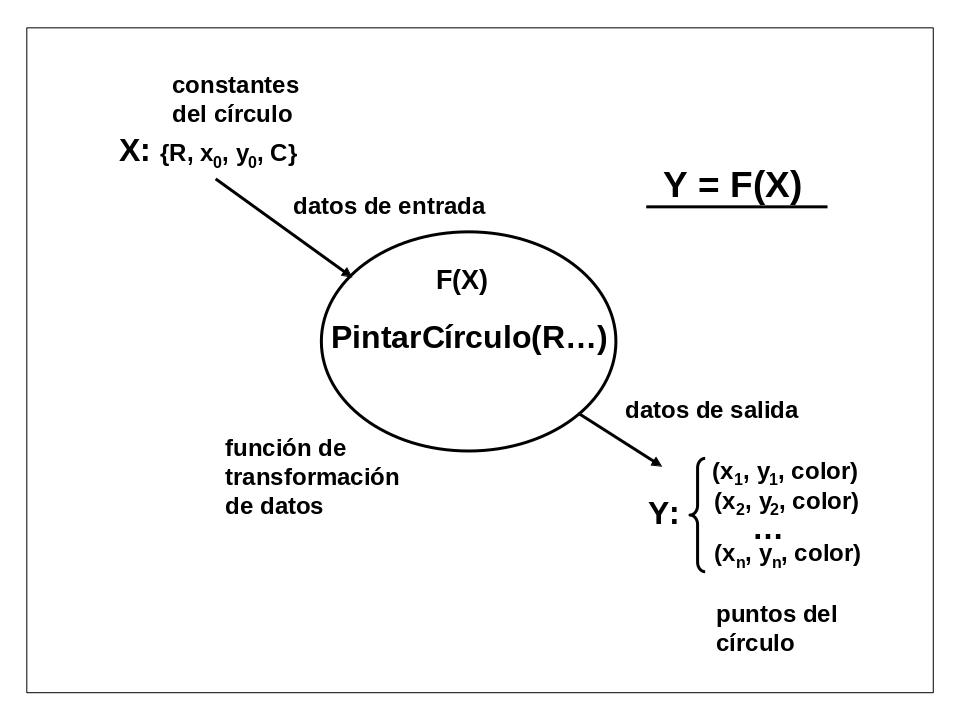
\includegraphics[width=0.5\textwidth]{images/fig12}
  \caption{Sistema software como función de transformación de datos}
  \label{fig:12}
\end{figure}

A este tipo de esquema se le denomina \emph{diagrama de flujo de
  datos}. \textbf{El diagrama de flujo de datos es un esquema asíncrono}
(no expresa secuencias); las flechas sólo indican los flujos de datos,
no el orden de ejecución.

\vspace{5mm}

El principal problema del enfoque estructurado es latente en el
momento en el que queremos añadir más elementos e interactuar con
ellos, por ejemplo, pintar varios círculos y actuar sobre los mismos
de forma selectiva, digamos borrar el segundo que se pintó.  Podríamos
hacer un bucle para crear n círculos, pero si queremos guardarlos
tendríamos que añadir tantas variables como círculos, con el objetivo
de retener cada conjunto de constantes. Este sistema es una
duplicación del sistema para solo un caso.

\vspace{5mm}

La disgregación de los conceptos en datos y funciones tiene sus pros y
sus contras, por ejemplo, este enfoque permite trabajar directamente
con la idea de base de datos o archivo, lo cual puede ser
beneficioso. Sin embargo, esta disociación implica \textbf{disminuir
  nuestro nivel de abstracción}.
\subsection{Enfoque orientado a objetos}
\label{sec:orgab1dc13} El enfoque orientado a objetos es la forma
particular de pensar el software en términos de elementos que
colaboran entre sí para realizar tareas.  Este enfoque nos da un nivel
de abstracción superior al estructurado, asociando cada elemento del
problema a un elemento software.  Cada elemento software tiene las
propiedades íntegras de cada elemento del discurso (lo que \emph{hace
  a una cosa ser una cosa}).
\subsubsection{Ejemplo: Pintar un círculo}
\label{sec:orge1a8962} En el ejemplo anterior, definimos un objeto
\texttt{círculo} que cumple las propiedades de un círculo según la
definición que hemos adaptado para nuestro sistema (en este caso, el
objeto contiene un centro y un radio) y tiene los mecanismos para
pintarse y crearse como elemento.

El enfoque de objetos piensa:
\begin{itemize}
\item En variables software capaces de recordar las constantes de un
  círculo, capaces de pintar un círculo y capaces de crearse a sí mismas
  como variables.
\item En el sistema software en términos de la interacción de estas
  variables, dadas sus respectivas capacidades para ejecutar
  operaciones, es decir, cómo relacionar todas las variables para
  conseguir que se realice la tarea de pintar círculos.
\end{itemize}

\begin{figure}[ht!]  \centering
  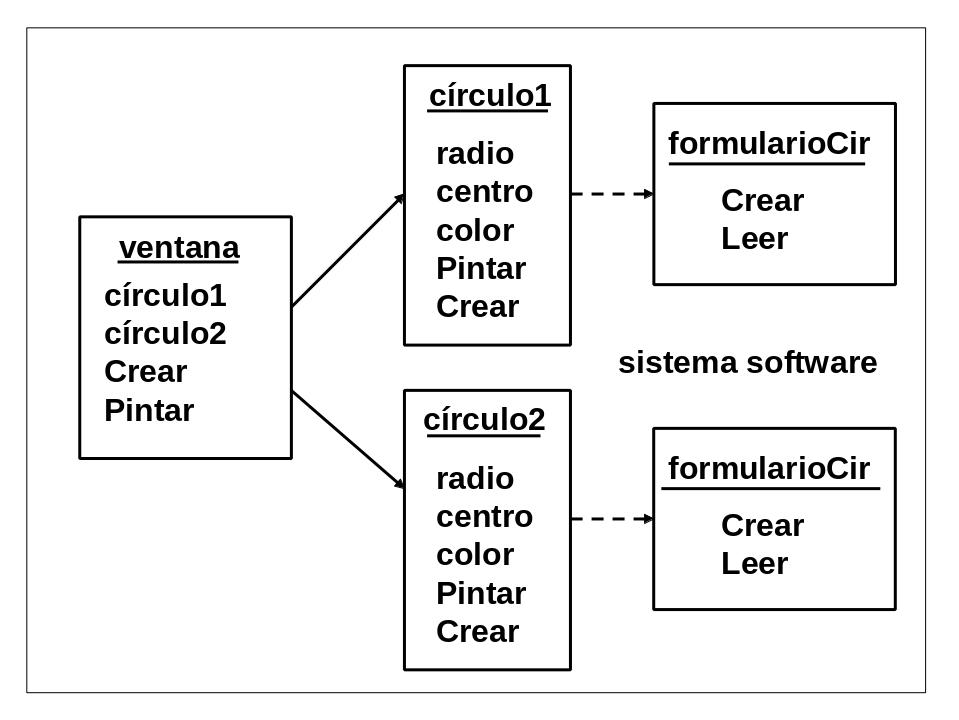
\includegraphics[width=0.5\textwidth]{images/fig18}
  \caption{Sistema software con enfoque de objetos}
  \label{fig:18}
\end{figure}

Este esquema muestra el sistema software, donde se aprecian las
relaciones entre las variables software que ejecutan la tarea de
pintar un círculo.  Como vemos, el sistema software, aun aplicando el
mismo algoritmo, tiene una organización diferente, y por tanto sus
propiedades también varían.
\subsection{Objetos}
\label{sec:org2b984f4} Esto que hemos ido llamando \emph{variables
  software} se conocen en este enfoque como \textbf{objetos}, y amplían
la idea de la variable software tratada en el enfoque estructurado, ya
que tienen capacidad de expresar cualquier cosa, incluso operaciones.
Otra definición complementaria de objeto es la siguiente: \emph{Un
  objeto es un elemento software cualitativamente distinto capaz de
  expresar un concepto más amplio, más ambiguo: cosa.}

\vspace{5mm}

Los objetos interactúan entre ellos mediante \textbf{mensajes},
solicitudes a objetos para que ejecuten operaciones.  Una buena
analogía de objetos y mensajes es el teatro, los objetos son
\emph{actores} y los mensajes son \emph{su diálogo}; el programa
describe a los actores, lo que tienen que hacer y decir.

\subsubsection{Propiedades de los objetos} Los objetos son definidos
por su nombre, asociado con una dirección de la memoria de la máquina.
Esta definición puede considerar además las propiedades que,
generalmente, se clasifican en \emph{atributos y operaciones}, también
denominadas \emph{métodos}.
\begin{itemize}
\item \textbf{Atributo:} Propiedad de un objeto, que está compuesto
  por un objeto o por una variable software tradicional. Los lenguajes
  OOP puros (como SmallTalk) solo admiten objetos como atributos, pero
  los lenguajes híbridos (como Java) también admiten variables software
  tradicionales.
\item \textbf{Operación: } Propiedad de un objeto que expresa su
  capacidad para ejecutar la rutina indicada por la misma. Las
  operaciones representan cualquier código capaz de ejecutar acciones.
\end{itemize}

\vspace{5mm}

Los lenguajes de programación acostumbran a distinguir los atributos
de las operaciones para elevar la eficiencia de compilación, pero en
principio, \textbf{no hay razón para distinguirlos}.

\vspace{5mm}

\paragraph{Globalidad de los atributos y operaciones:} Los atributos
de un objeto son globales para todas las operaciones del mismo. Esto
es, cualquier línea de código de cualquier método de un objeto tiene
acceso inmediato a todos los atributos del propio objeto. Esto
facilita el acceso a los atributos, pero tiene los siguientes
inconvenientes:
\begin{itemize}
\item Cuando una operación de un objeto quiere usar otra operación del
  mismo, esta operación no conoce cómo usarla, ya que en la cabecera de
  la operación llamada no se refleja la relación con los atributos del
  objeto, y podría interceder en el uso de los atributos de la operación
  llamante.\footnote{Mutabilidad en los atributos del objeto.}
\item Al modificar alguna línea de código de una operación debemos
  revisar todas las líneas de código de todas las operaciones, ya que
  cambiar el comportamiento de una operación que a priori puede ser
  necesaria para el resto de operaciones podría desencadenar en un mal
  funcionamiento del objeto.
\end{itemize}

\vspace{5mm}

\paragraph{Visibilidad de los atributos y operaciones:} Los objetos
son, de una forma coloquial, \emph{parcelas bien definidas};
accesibles desde dentro pero no tan fácilmente desde fuera. El acceso
desde fuera está regulado por un "control de visibilidad".
Los elementos designados como \emph{públicos} son accesibles a todos
los objetos del sistema software. Los \emph{privados} son accesibles
sólo desde el propio objeto.

\subsubsection{Sobre la ambigüedad} Una de las característica más
importantes del enfoque orientado a objetos es la capacidad de éstos
para expresar alternativas o significados diversos, lo que comúnmente
llamamos \textbf{ambigüedad}.

\vspace{5mm}

El enfoque estructurado utiliza dato y función de transformación de
datos como elementos del sistema software, mientras el enfoque de
objetos utiliza los elementos objeto, con el significado de
\emph{cosa}, y mensaje con el significado de solicitud de servicio a
una variable.  El significado ambiguo de \emph{cosa} que tienen los
objetos nos permite hacer un diseño estructurado con aspecto (ropaje?)
de objetos, pero no al contrario (diseño de objetos con aspecto
estructurado).

\vspace{5mm}

\textbf{El enfoque de objetos se acomoda mejor a la diversidad de
  problemas que aborda el software.}  Los objetos son más tolerantes
para expresar la idea general de función que el enfoque estructurado,
el cual está obligado a expresar esa función en términos de “entrada,
proceso y salida”.  No obstante, esta mayor libertad de expresión
tampoco es gratis siempre. A menudo hay que aceptar cualidades
“extrañas” como la capacidad de pintarse, ampliarse, moverse,
borrarse, etc.  que tienen los círculos software, para ajustarse al
enfoque.

\vspace{5mm}

La \textbf{ambigüedad del enfoque de objetos} también facilita que un
\textbf{elemento software}, por sí solo, \textbf{exprese completamente
  un concepto}, por ejemplo círculo, mientras que el enfoque
estructurado obliga, muchas veces, a disociarlos en funciones y datos.


\begin{figure}[ht!]  \centering
  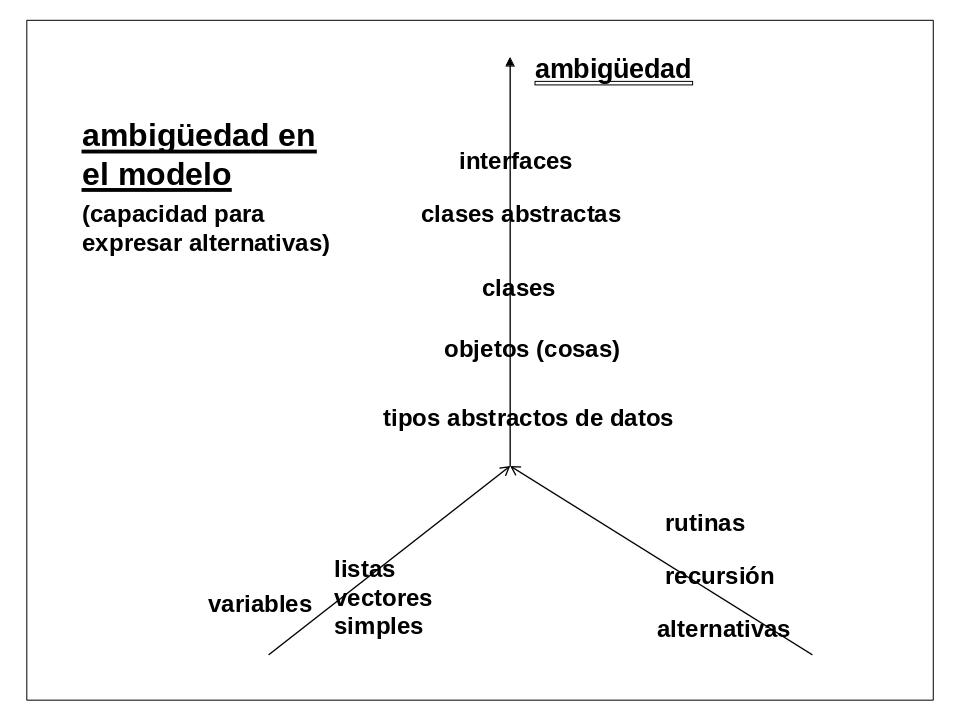
\includegraphics[width=0.5\textwidth]{images/fig111}
  \caption{Aumento de la capacidad de ambigüedad en elementos
    software}
  \label{fig:111}
\end{figure}

La figura muestra la evolución del software hacia el aumento de la
ambigüedad de sus elementos primarios.  También nos muestra claramente
qué es un TAD, es decir, un \emph{tipo abstracto de datos}. Estos TAD
\textbf{no se consideran objetos}, ya que, a diferencia de éstos,
siempre deben ser datos (un objeto no tiene por qué ser un dato, puede
ser cualquier cosa, no está comprometido a desempeñar dicha función ni
ninguna en particular).

\subsubsection{Objetos vs Realidad} Gracias a la mayor capacidad
expresiva de los objetos se dice a menudo que los objetos reflejan
mejor la realidad.  Pero esta idea perjudica, más que beneficia porque
reflejar la realidad:
\begin{itemize}
\item No es el propósito de los sistemas software, salvo que sean de
  simulación.
\item Dificulta los cambios en los sistemas software.
\item ¿Qué significa? La realidad varía según el espectador.
\end{itemize}

\subsubsection{Refactorización}
Se llama \emph{refactorización} a los procesos que \textbf{modifican
  el sistema para mejorar alguna cualidad interna sin alterar sus
  funciones}. A diferencia de la forma tradicional, que aspira
a alcanzar un diseño perfecto, la refactorización acepta que el
objetivo es funcionar a tiempo, y que después de probarlo se podrá
mejorar el funcionamiento del sistema software.

\subsubsection{Encapsulado y principio de ocultación}
Como un objeto es una \emph{parcela de software}, se suele decir que
un objeto \textbf{encapsula} sus atributos y operaciones, lo cual es
correcto, no distorsiona nuestra analogía con la parcela. No obstante,
cuando se asocia encapsulado con ocultación de información tenemos un
problema.

Es cierto que el enfoque de objetos facilita algunas formas de
desarrollo de software, como los prototipos evolutivos y el diseño en
paralelo, pero no son facilidades intrínsecas.\\
\textbf{El principio de ocultación establece que:}
\begin{itemize}
\item Cada módulo es independiente del código de la implementación
  de los demás (los clientes se comunican con los servicios por
  medio de interfaces, que permiten realizar las operaciones sin
  conocimiento de la modificación del código anteriormente
  mencionado).
\item La interfaz o definición de cada módulo debe revelar lo menos
  posible del trabajo interno del módulo.
\end{itemize}

\newpage

\subsection{Representación gráfica de los objetos}
En este apartado veremos varios tipos de gráficos para representar
objetos, sus atributos, operaciones y la interacción entre ellos (es
decir, los mensajes).
\subsubsection{UML (Unified Modelling Language)}
UML es un sistema de símbolos y diagramas (un lenguaje) que sirve para
expresar (modelar) los diseños de los sistemas software. La palabra
unificado refleja el acuerdo de sus autores.

\paragraph{Objetos:}
UML representa a los objetos mediante \textbf{cajas}. Si se usa la
definición extendida de objeto, la caja marca tres zonas: la superior
contiene, subrayado, el nombre del objeto; la zona central contiene
los atributos y la inferior los métodos u operaciones. En caso de usar
la definición compacta de objeto, la caja solo contiene la zona
superior. En UML los elementos públicos son diferenciados de los
privados según el símbolo que precede su nombre; \textrm{+} para los públicos
y \textrm{-} para los privados.

\begin{figure}[ht!]  \centering
  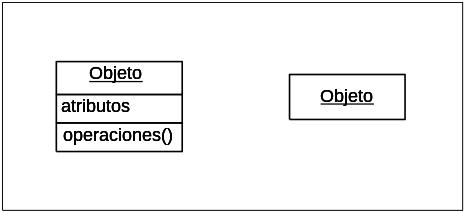
\includegraphics[width=0.5\textwidth]{images/fig21}
  \caption{Representación de un objeto en UML}
  \label{fig:21}
\end{figure}

\vspace{5mm}

\paragraph{Mensajes:}
UML representa los mensajes mediante líneas dirigidas etiquetadas con
el nombre de su operación, \textbf{desde el llamante al llamado}.

\begin{figure}[ht!]  \centering
  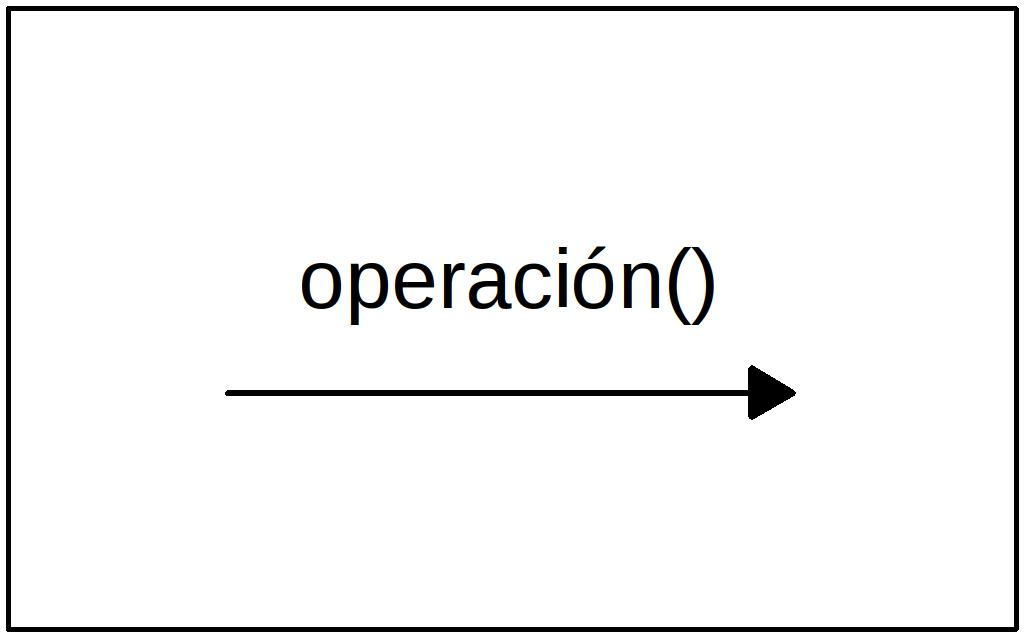
\includegraphics[width=0.3\textwidth]{images/fig22}
  \caption{Representación de un mensaje en UML}
  \label{fig:22}
\end{figure}

\paragraph{Diagrama de secuencias:}
Los objetos que participan en la interacción se dibujan,
horizontalmente, en la parte superior del diagrama a través de sus
esquemas simplificados (cajas conteniendo sólo el nombre
subrayado). Debajo de cada objeto se dibuja una línea vertical
discontinua llamada línea de vida que indica, en el eje tiempo, la
existencia del objeto.
Los mensajes se colocan entre las líneas de vida de los objetos,
siguiendo la secuencia de ejecución. Si se quiere resaltar la
devolución de algún valor, se puede dibujar una flecha discontinua
apuntando hacia el objeto emisor, etiquetada con el nombre del valor
de retorno.

\begin{figure}[ht!]  \centering
  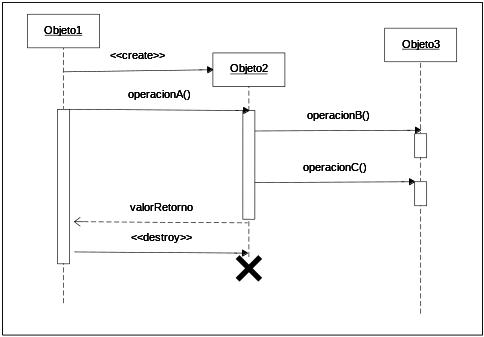
\includegraphics[width=0.5\textwidth]{images/fig23}
  \caption{Diagrama de secuencias en UML}
  \label{fig:23}
\end{figure}

Para indicar la creación o destrucción de un objeto se utilizan,
respectivamente, las etiquetas estereotipadas \textrm{<<create>>} y
\textrm{<<destroy>>} en el mensaje que se le envía al objeto. La
creación de un objeto se distingue dirigiendo el mensaje a la caja que
representa al objeto. La destrucción de un objeto se muestra dibujando
una X grande al final de su línea vida.
\newpage
\paragraph{Diagrama de colaboración:}
Un diagrama de colabroación es un diagrama de interacción que resalta
la organización de los objetos que envían y reciben los mensajes. Este
diagrama muestra un conjunto de objetos, los enlaces entre ellos y los
mensajes que intercambian.\\
\textbf{Un enlace es una instancia de una asociación o dependencia entre
  clases.} Se representa con una línea continua que une los dos
objetos.

\begin{figure}[ht!]  \centering
  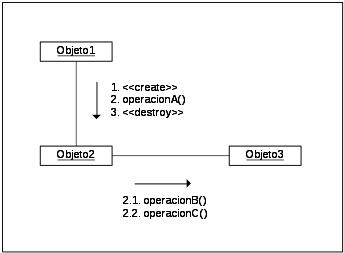
\includegraphics[width=0.5\textwidth]{images/fig25}
  \caption{Diagrama de colaboración en UML}
  \label{fig:25}
\end{figure}

Los mensajes se escriben junto a los enlaces, indicando el sentido con
una flecha que apunta hacia el receptor y numerándolos para expresar
el orden de ejecución. \\
El diagrama de colaboración ofrece una vista de conjunto de estructura
y funcionamiento, pero incide en la estructura, afectando a la
claridad del funcionamiento (toca seguir la secuencia de mensajes
saltando de una línea a otra, buscando la numeración).\\
Además, esta forma de representación dificulta la modificación del
diseño, por lo que interesa usar este diagrama cuando no interese
demasiado seguir el funcionamiento y se esperen pocas modificaciones
del diseño.

\subsection{Clases}
Una \textbf{clase} es una definición intensiva de un conjunto de
objetos. Establece las propiedades distitntivas de cualquier elemento
del conjunto que define.\\

\vspace{5mm}

Considerando las clases se podría decir que un objeto es una
\textbf{instancia} de una clase o un elemento del conjunto definido
por una clase. La notación UML de un objeto en particular, teniendo en
cuenta la clase a la que pertenece, es \texttt{objeto:clase}. Si se
quiere expresar un objeto cualquiera (anónimo) de una clase, la
notación sería \texttt{:clase}.

\vspace{5mm}

Las clases enriquecen el enfoque de objetos. Un objeto es una cosa y
una clase define un conjunto de cosas con iguales propiedades, pero
valores distintos, por tanto las clases establecen una generalización,
una \textbf{abstracción} mayor que los objetos. La \textbf{estructura y
  relaciones de los elementos del sistema} software se pueden pensar en
términos de las \textbf{clases}, y dejar los objetos para pensar los diseños
dinámicos particulares del sistema.

\vspace{5mm}

La representación de las clases y los objetos coinciden prácticamente
en el lenguaje UML, con la salvedad de que el nombre de las clases no
se subraya.

\subsubsection{Diagrama de clases}
El diagrama de clases expresa la estructura u organización del sistema
software en términos de las clases. Además de intervenir en el
funcionamiento, el diseño del diagrama es clave porque expresa la
organización del sistema, y ésta decide sobre aspectos fundamentales:
significado, facilidad de desarrollo en paralelo y faciidad de modificación.

\begin{figure}[ht!]  \centering
  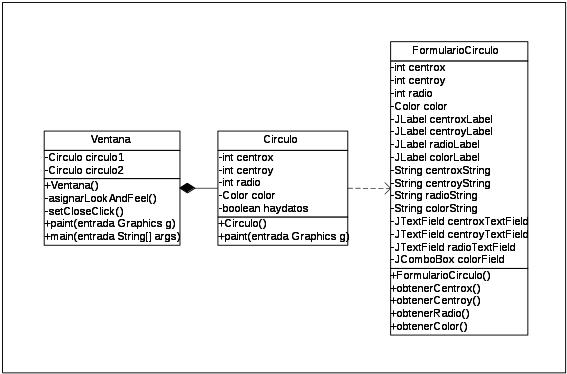
\includegraphics[width=0.5\textwidth]{images/fig33}
  \caption{Diagrama de clases en UML}
  \label{fig:33}
\end{figure}

La figura muestra el diagrama de clases del sistema para dibujar
círculos. Se aprecian las clases, los elementos que componen cada
clase y las relaciones entre las clases, así como la visibilidad de
dichos elementos.\\
El diagrama de clases complementa a los diagramas de secuencias,
muestra la forma del soporte de los mecanismos, mientras que los
diagramas de secuencias muestran el funcionamiento parcial de los
mecanismos.
\begin{figure}[ht!]  \centering
  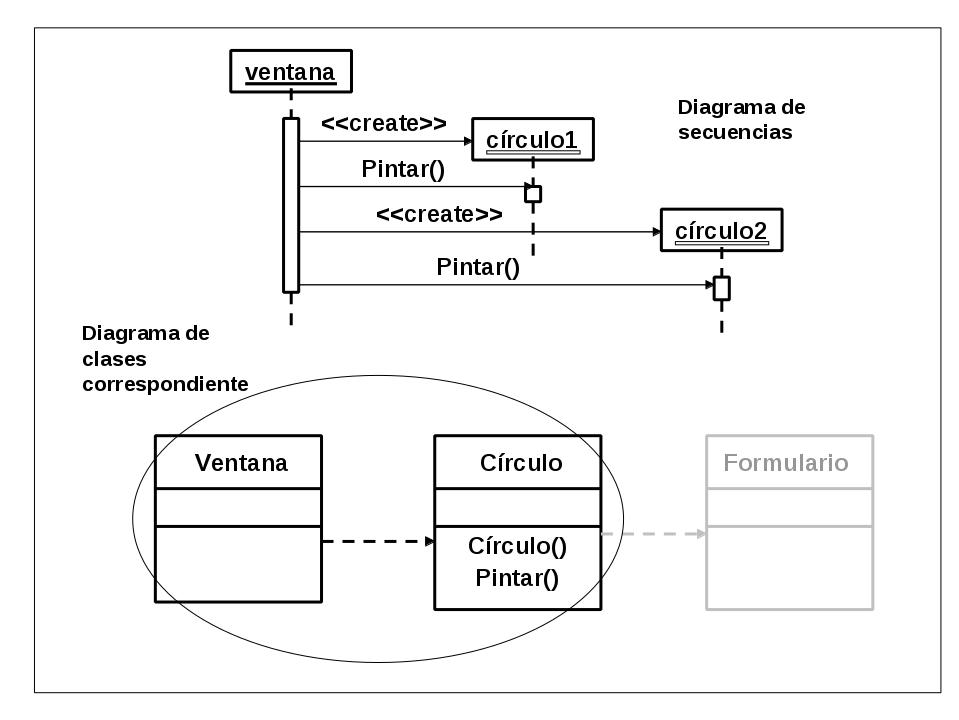
\includegraphics[width=0.5\textwidth]{images/fig34}
  \caption{Correspondencia entre diagrama de clases y de secuencias en UML}
  \label{fig:34}
\end{figure}

El diagrama de secuencias define el funcionamiento parcial del
mecanismo para pintar círculos y el diagrama de clases correspondiente
describe la organización de los elementos del sistema en términos de
los conjuntos y sus relaciones.

\subsubsection{Relaciones entre clases}
El enfoque de objetos acepta cuatro tipos de relaciones entre elementos:
\paragraph{Dependencia:}
Se denomina \emph{relación de dependencia} a la relación de una clase
hacia otra cuando \textbf{los objetos de la primera usan objetos de la
  segunda}. Esta relación es direccional. \\
En UML la relación de dependencia se representa con una flecha
discontinua del elemento dependiente A hacia el elemento independiente
B (del que usa hacia el usado).
\paragraph{Asociación:}
Se denomina \emph{relación de asociación} a la relación de una clase
hacia otra cuando \textbf{los objetos de la primera contienen
  atributos que son objetos de la segunda clase}. \\
En UML la asociación unidireccional se representa con una flecha
continua de la clase que contiene a la clase cuyos objetos son
contenidos. La asociación bidireccional se representa con una línea
continua entre las clases asociadas.
\paragraph{Agregación:}
Se denomina \emph{relación de agregación} entre clases cuando hay una
\textbf{relación “todo/parte” entre los objetos de ambas clases}. \\
En UML se utiliza una línea continua y un rombo hueco en el lado del
continente para representar una relación de agregación. \\
La relación de agregación introduce conceptualmente una estructura
jerárquica del tipo `está formado por` en el diagrama de clases, lo
cual la diferencia de las relaciones anteriormente mencionadas (que
son entre iguales).
\paragraph{Composición:}
La \emph{composición} es otra forma de agregación con una fuerte
relación de pertenencia: Un objeto “parte” sólo pertenece a un objeto
“todo” y cuando se destruye el objeto “todo” se destruye el o los
objetos “parte”. \\
En la composición el objeto “todo” controla la disposición y vida de
las partes. Hay un cierto efecto transitivo: lo que le ocurre al todo
le debe ocurrir a las partes. En UML se utiliza una línea continua y
un rombo relleno en el lado del continente.
\subsubsection{Herencia}
Desde el punto de vista formal, se establece que: \\
La \emph{herencia} es una relación entre clases donde una de ellas
comparte la estructura o comportamiento definido en una (herencia
simple) o más clases (herencia múltiple). Las subclases pueden compartir
atributos y operaciones de sus superclases, y también redefinir
algunos de estos elementos. \\
Tenemos que tener mucho cuidado con la herencia, ya que, como ya hemos
visto, generar dependencias fuertes es malo para el mantenimiento y la
modificación de nuestro diseño software. \\
En un UML, la herencia se denota siempre desde la subclase a la
superclase, con un triángulo hueco a la superclase.
\subsubsection{Polimorfismo}
El polimorfismo es una de las cualidades más importantes del enfoque
de objetos por su aporte a la ambigüedad en el diseño. Se asocia con
el mecanismo de herencia y permite que la operación definida con la
misma cabecera sea implementada de maneras distintas.  Formalmente, se
denomina polimorfismo a la \textbf{capacidad de una operación para manifestar
  un comportamiento diferente dependiendo del objeto que la ejecuta.}
\subsubsection{Principio de sustitución de Liskov}
Después del análisis de los muchos problemas de la herencia, el
principio de sustitución de Liskov, formulado hace casi dos décadas,
ofrece un camino útil y confiable para aprovechar los favores de la
herencia.  Literalmente el principio define, en términos de una
sustitución segura, cuando una subclase es un subtipo de una
superclase.  \\
\emph{“Si para cada objeto O1 de tipo S hay un objeto O2 de tipo T tal
  que para todos los programas P definidos en términos de T, el
  comportamiento [interno] de P no cambia cuando O1 es sustituido por
  O2, entonces S es un subtipo de T.”} \\
Pero lo interesante es ver el principio de sustitución desde otra
perspectiva.  \emph{La herencia permite sustituir un objeto por otro,
  es decir cambiar una tarea por otra, sin riesgo, siempre que las
  subclases sean subtipos de las superclases.}  \\
El cumplimiento del principio de sustitución exige que los métodos de
las clases derivadas deban mantener las siguientes relaciones con los
métodos de la clase base:
\begin{itemize}
\item La clase derivada debe tener un método correspondiente a cada
  método de la clase base. Este método puede heredarse directamente de
  la clase base o sobrescribirse.
\item Cada método de la clase derivada que se corresponda a un método
  de la clase base debe requerir lo mismo o menos que la clase
  base. Es decir, si se sobrescribe un método heredado de la clase
  base, las precondiciones del método deben ser más débiles o
  permisivas que las del método de la clase base. El nuevo método no
  puede ser más restrictivo que el método heredado.
\item Cada método de la clase derivada que se corresponda a un método
  de la clase base debe garantizar lo mismo o más que la clase
  base. Es decir, si se sobreescribe un método heredado de la clase
  base, las postcondiciones del método de las clases derivada deben
  ser más fuertes o rigurosas que las heredadas de la clase
  base. Dicho de otro modo, el método de la clase derivada no debe
  comprometerse a ofrecer mayores resultados o resultados diferentes;
  sólo debe comprometerse a hacer lo que hace el método de la clase
  base, garantizando también las propiedades adicionales. Por ejemplo,
  si un método de la clase base devuelve un número mayor que el
  argumento que recibe, un método de una clase derivada podría
  devolver un número primo mayor que el argumento. Pero no estaría
  permitido que el método de la clase derivada devolviese un número
  menor o igual que el argumento.
\item Está permitido que la clase derivada introduzca nuevos métodos
  adicionales que no aparezcan en la clase base.
\end{itemize}
\subsubsection{Clases abstractas}
Se denomina \emph{método abstracto} al método que sólo expresa la
cabecera y carece de código interno. Dicho de otro modo, un método que
está declarado pero no implementado. \\
Se denomina \emph{clase abstracta} a la clase que contiene al menos un
método abstracto porque refleja la abstracción de ese método. Por
ejemplo, la clase Figura. También se les llama clases virtuales o
diferidas.
